\documentclass[12pt]{article}
\usepackage[margin=1.5in]{geometry}
\usepackage{libertine}
\usepackage{cite}
\usepackage{booktabs}   %% For formal tables:
                        %% http://ctan.org/pkg/booktabs
\usepackage{subcaption} %% For complex figures with subfigures/subcaptions
                        %% http://ctan.org/pkg/subcaption
\usepackage{catchfilebetweentags} %% For importing code snippets
\usepackage{lineno} %% For line numbers on code snippets
\usepackage{pgfplots}
\usepackage{multicol}
\usepackage{fancyvrb}
\usepackage{wrapfig}
\usepackage{minted}
\usepackage{tikz-cd}
\usepackage{csquotes}
%%%%%%%%%%%%%%%%%%%%%%%%%%%%%%%%%%%%%%%%%%%%%%%%%%%%%%%%%%%%%%%%%%%%%%%%%%%%%%%%
%% Agda special Characters
%%%%%%%%%%%%%%%%%%%%%%%%%%%%%%%%%%%%%%%%%%%%%%%%%%%%%%%%%%%%%%%%%%%%%%%%%%%%%%%%
\usepackage{amssymb}
\usepackage{turnstile}
\usepackage{bbm}
\usepackage[greek, english]{babel}
\usepackage{MnSymbol}
\usepackage{stmaryrd}
\usepackage{csquotes}
\newcommand\doubleplus{+\kern-1.3ex+\kern0.8ex}
\newcommand\mdoubleplus{\ensuremath{\mathbin{+\mkern-8mu+}}}
\makeatletter
\newcommand\incircbin
{%
  \mathpalette\@incircbin
}
\newcommand\@incircbin[2]
{%
  \mathbin%
  {%
    \ooalign{\hidewidth$#1#2$\hidewidth\crcr$#1\bigcirc$}%
  }%
}
\newcommand{\oeq}{\ensuremath{\incircbin{=}}}
\makeatother
\makeatletter
\newcommand\insquarebin
{%
  \mathpalette\@insquarebin
}
\newcommand\@insquarebin[2]
{%
  \mathbin%
  {%
    \ooalign{\hidewidth$#1#2$\hidewidth\crcr$#1\bigbox$}%
  }%
}
\newcommand{\sqtri}{\ensuremath{\insquarebin{\triangle}}}
\makeatother
\usepackage{ucs}
\DeclareUnicodeCharacter{8759}{\ensuremath{\squaredots}}
\DeclareUnicodeCharacter{951}{\textgreek{\texteta}}
\DeclareUnicodeCharacter{737}{\ensuremath{^\text{l}}}
\DeclareUnicodeCharacter{691}{\ensuremath{^\text{r}}}
\DeclareUnicodeCharacter{7523}{\ensuremath{_\text{r}}}
\DeclareUnicodeCharacter{8343}{\ensuremath{_\text{l}}}
\DeclareUnicodeCharacter{8718}{\ensuremath{\blacksquare}}
\DeclareUnicodeCharacter{957}{\textgreek{\textnu}}
\DeclareUnicodeCharacter{961}{\textgreek{\textrho}}
\DeclareUnicodeCharacter{929}{\textgreek{\textRho}}
\DeclareUnicodeCharacter{954}{\textgreek{\textkappa}}
\DeclareUnicodeCharacter{10214}{\ensuremath{\lsem}}
\DeclareUnicodeCharacter{10215}{\ensuremath{\rsem}}
\DeclareUnicodeCharacter{8857}{\mdoubleplus}
\DeclareUnicodeCharacter{8860}{\oeq}
\DeclareUnicodeCharacter{9043}{\ensuremath{\sqtri}}
\DeclareUnicodeCharacter{928}{\textgreek{\textPi}}
\DeclareUnicodeCharacter{922}{\textgreek{\textKappa}}
\DeclareUnicodeCharacter{931}{\textgreek{\textSigma}}
\DeclareUnicodeCharacter{916}{\textgreek{\textDelta}}
\DeclareUnicodeCharacter{921}{\textgreek{\textIota}}
\DeclareUnicodeCharacter{8779}{\ensuremath{\backtriplesim}}
\DeclareUnicodeCharacter{8799}{\ensuremath{\stackrel{?}{=}}}
\DeclareUnicodeCharacter{10181}{\ensuremath{\lbag}}
\DeclareUnicodeCharacter{10182}{\ensuremath{\rbag}}
\DeclareUnicodeCharacter{8760}{\ensuremath{-}}
\usepackage[references]{agda}

\newcommand{\Nat}{\AgdaDatatype{ℕ}}
\newcommand{\Int}{\AgdaDatatype{ℤ}}
%%%%%%%%%%%%%%%%%%%%%%%%%%%%%%%%%%%%%%%%%%%%%%%%%%%%%%%%%%%%%%%%%%%%%%%%%%%%%%%%

\newtheorem{principle}{Principle}
\usepackage{authblk}


\title{Automatically and Efficiently Illustrating Polynomial Equalities in Agda}
\author{
  Donnacha Ois\'in Kidney \\ \vspace{3cm}
  Supervisor: Professor Gregory Provan \\ \vspace{3cm}
  Final-Year Project---BSc in Computer Science \\ \vspace{3cm}
  Department of Computer Science \\
  University College Cork
}

\begin{document}
\maketitle
\pagebreak
\begin{abstract} \textbf{
  We present a new library which automates the construction of equivalence
  proofs between polynomials over commutative rings and semirings in the
  programming language Agda \cite{norell_dependently_2008}. It is significantly
  faster than Agda's existing solver. We use reflection to provide a simple
  interface to the solver, and demonstrate how to use the constructed proofs to
  provide step-by-step solutions.}
\end{abstract}
\newpage
\section{Declaration of Originality}
In signing this declaration, you are conforming, in writing, that the submitted
work is entirely your own original work, except where clearly attributed
otherwise, and that it has not been submitted partly or wholly for any other
educational award.

I hereby declare that:
\begin{itemize}
  \item this is all my own work, unless clearly indicated otherwise, with full
    and proper accreditation;
  \item with respect to my own work: none of it has been submitted at any ed-
    ucational institution contributing in any way to an educational award;
  \item with respect to another’s work: all text, diagrams, code, or ideas,
    whether verbatim, paraphrased or otherwise modified or adapted, have been
    duly attributed to the source in a scholarly manner, whether from books,
    papers, lecture notes or any other student’s work, whether published or
    unpublished, electronically or in print.
\end{itemize}
\begin{tabular}{@{}p{.5in}p{4in}@{}}
Signed: & \hrulefill \\
Date: & \hrulefill \\
\end{tabular}
\newpage

A version of this work has been submitted for publication to the International
Conference on Functional Programming.
\newpage
\tableofcontents
\newpage

\section{Introduction}
\subsection{Background}
\paragraph{The Foundational Crisis}
In the early 20th century, the foundations of mathematics began to crumble.
The first crack was Russell's paradox, discovered in 1901.
Similar paradoxes soon followed: each represented core errors in the
foundational theories that had underpinned all of mathematics up until that
point.

The work of papering over these cracks began in earnest:
Russell himself (along with Whitehead) published the Principia Mathematica (PM)
\cite{whitehead_principia_1910}, a
formalisation of contemporary mathematics based on a theory that accounted for
the discovered paradoxes.
The task proved to be far more difficult than was anticipated: the PM was
infamously verbose (350 pages of preparation precede the proof that \(1+1=2\)),
and both men eventually gave up before reaching their goal of a full
formalisation.

These repeated attempts and failures to shore up the foundations of mathematics
became known as the ``Foundational Crisis''.
There were three competing schools of thought on how to address the crisis:
Russell and Whitehead belonged to the logicism camp, although this came to be
overshadowed by the other two philosophies.
David Hilbert championed the ``formalists'', the leading school of thought at
the time.
These mathematicians envisioned a solution to the crisis in the form of a
finite set of axioms, satisfying a set of requirements (here simplified):
\begin{description}
  \item[Completeness] Any true statement can be derived from the axioms.
  \item[Consistency] No untrue statement can be derived from the axioms.
  \item[Decidability] Any statement can be decided as true or false using an
    algorithm.
\end{description}
These requirements became known as Hilbert's program.

While intended to be a scaffolding on which to rebuild, these requirements acted
more as targets for later attacks.
Firstly, in 1931, Gödel published his incompleteness theorems
\cite{godel_uber_1931}, which proved that the first two requirements
(completeness and consistency) were \emph{impossible} to achieve.
And finally, in 1936, Alonzo Church and Alan Turing independently showed that
the Entscheidungsproblem was unsolvable \cite{church_unsolvable_1936,
  church_._1937}, showing that the third requirement was also impossible to
satisfy.

\paragraph{Intuitionism}
Among the rubble stood intuitionism: the third school of thought, once maligned,
now was more attractive in light of the failure of Hilbert's program.
Formalists and intuitionists had deep philosophical disagreements: the formalist
held that mathematics was the pursuit of external truth.
Hilbert, in particular, insisted that the axioms and rules of a mathematical
formalism were not arbitrary:
\blockquote[David Hilbert \cite{hilbert_natur_1992}]{
  We are not speaking here of arbitrariness in any sense. Mathematics is not
  like a game whose tasks are determined by arbitrarily stipulated rules.
  Rather, it is a conceptual system possessing internal necessity that can only
  be so and by no means otherwise.
}
Intuitionists, on the other hand, believed that mathematics was a pure
construct of the human mind, and had little or nothing to do with objective
reality.
Its main proponent was L. E. J. Brouwer, who became engaged in a bitter dispute with
Hilbert, eventually culminating in Brouwer's removal from the Mathematische
Annalen, on the basis of Hilbert's claim that his theories represented a
``danger to mathematics'' \cite{van_dalen_war_1990}.

In terms of nuts-and-bolts, the defining feature separating intuitionism from
classical logic is the absence of the law of the excluded middle, or ``choice'':
\begin{equation}
  \forall P. P \vee \neg P
\end{equation}
This axiom has a deep relation with constructiveness and computability.
Intuitionism is a constructive theory: to say that something is true is to say
that we have a proof of it.
Allowing this axiom, then, would imply that once we could state a theorem
intuitionistically, we would be able to pluck---either from thin air or from an
algorithm---a proof of its truth or falsehood.
But of course, via the Entscheidungsproblem, we know that this is impossible.

\paragraph{Intuitionistic Type Theory and Agda}
Intuitionism has had many incarnations since Brouwer (it gained widespread
popularity after Bishop), but the particular version of interest to us comes
from a strange source: the type systems of programming languages.
In formal terms, we are talking about the ``Curry-Howard isomorphism''
(Fig.~\ref{CH}): a way to bridge the world of programming languages and
formalised mathematics.

\begin{wrapfigure}{r}{0.5\textwidth}
  \centering
  \begin{tikzcd}
    \textit{Type}    \ar[r, Leftrightarrow] & \textit{Proposition}  \\
    \textit{Program} \ar[r, Leftrightarrow] & \textit{Proof}
  \end{tikzcd}
  \caption{The Curry-Howard Isomorphism}
  \label{CH}
\end{wrapfigure}
This brings us, at long last, to Agda, the subject of this work.
Agda is a programming language and intuitionistic theory based on Per
Martin-Löf's intuitionistic type theory \cite{martin-lof_intuitionistic_1980}.
Its syntax and evaluation strategy is similar to Haskell, but as a formalism it
can be used to prove mathematical statements.

\subsection{Our Contributions}
It is over a hundred years since the publication Principia Mathematica, and we are still a
long way away from formalising all of mathematics.
There is a popular website which tracks the progress of this formalisation
against the ``100 greatest theorems'' \cite{wiedijk_formalizing_2018}: at time
of writing, the number stands at 93.

There are many reasons for why we haven't managed to formalise all 100 yet:
chief among them is that, while we have come far from the days of the PM, proofs
are still verbose and tedious.

This work intends to alleviate some of the tedium of constructing a particular
kind of proof: identities over commutative rings.
We write a verified and proven library for automation in Agda, to automate the
construction of proofs like the one in Fig.~\ref{ring-proof}, making them as
simple as Fig.~\ref{the-solver}.

\begin{figure*}
  \centering
  \begin{subfigure}[b]{\textwidth}
    \centering
    \ExecuteMetaData[Introduction.tex]{lemma}
    \label{ring-lemma}
    \vspace{-10pt}
  \end{subfigure}
  \begin{subfigure}[b]{.5\textwidth}
    \ExecuteMetaData[Introduction.tex]{proof}
    \caption{A Tedious Proof}
    \label{ring-proof}
  \end{subfigure}%
  \begin{subfigure}[b]{.3\textwidth}
    \centering
    \ExecuteMetaData[Introduction.tex]{solver}
    \caption{Our Solver}
    \label{the-solver}
  \end{subfigure}
  \caption{Comparison Between A Manual Proof and The Automated Solver}
  \label{comparison}
\end{figure*}

The main contributions of our library are as follows:
\begin{description}
  \item[Ease of Use] Proofs like the one in Fig.~\ref{ring-proof} are long,
    difficult to write, and uninteresting. Our solver, in contrast, is extremely
    simple to use: the single line in Fig.~\ref{the-solver} solves the lemma.

    This interface (section~\ref{interface}) is implemented using a lightweight
    reflection system (section~\ref{reflection}), which does not require the user
    to write \emph{any} reflection code, even if they use the solver with their
    own custom type. 
  \item[Performance] Our solver is significantly faster than Agda's current ring
    solver, cutting type-checking time down from minutes to seconds in several
    use cases (section~\ref{benchmarks}).

    As described in \cite{gregoire_proving_2005}, we use a sparse internal
    representation of polynomials (section~\ref{sparse-opt}). However, because
    of differences between Agda and Coq's type checker, we found that this
    optimisation---on its own---did not deliver a significant speedup, and
    actually damaged performance in a number of cases. Achieving the performance
    we did required an entirely separate kind of optimisation, described in
    section~\ref{syntactic-unif}.
  \item[Pedagogical Solutions] Computer algebra systems (CASs) outside the
    rigorous world of dependently-typed languages do far more than just check
    proofs for mistakes: they have a wealth of other features which can help
    with learning mathematics as well as verifying it.

    We hope that similar systems developed in Agda can do the same: as a
    demonstration, we implement ``step-by-step solutions'', one of the most
    popular features of modern CASs. Far from being ill-suited to Agda, we show
    that the constructive nature of our proofs allows for a natural
    implementation (section~\ref{pedagogical}).
\end{description}
\subsection{Scope}
In this section, we will explain the intended uses and necessary limitations of
the solver.

\begin{description}
  \item[Equivalences] First, an inflexibility: the solver deals very
    specifically with the domain of \emph{equivalence} proofs, like the one in
    Fig.~\ref{comparison}. While it may be of use in other settings (finding
    roots, etc.), that is not explored here.
  \item[Setoids] On the other hand, we are very flexible about what kind of
    ``equivalence'' we prove. In fact, the solver will work with any equivalence
    relation, as long as it comes with proofs of the relevant ring axioms. This
    is useful for all of the usual things (approximating quotients and so on),
    but it also provides the basis for our ``step-by-step solutions''
    implementation in section~\ref{pedagogical}.
  \item[Almost Rings] As in \cite[section~5]{gregoire_proving_2005}, we use a
    peculiar algebraic structure which lies somewhere between a semiring and a
    ring. These ``almost-rings'' have all of the usual laws of a commutative
    ring, but instead of demanding additive inverses, they require the
    comparatively permissive ``pseudo-inverse'' operation, which obeys the
    following equations:
    \begin{align}
      \vspace{-10pt}
      -(x * y)    &= - x * y \label{ringmul} \\
      -(x + y)    &= -x + -y \label{ringadd}
    \end{align}
    This allows the solver to work on types which don't have an additive inverse
    (like \(\Nat\)): such types just supply the identity function instead of
    negation, and the two laws above are satisfied.

    A potential worry is that because we don't require \(x + -x = 0\)
    axiomatically, it won't be provable in our system. Happily, this is not the
    case: as long as \(1 + -1\) reduces to \(0\) in the coefficient set, the
    solver will verify the identity.
  \item[Weak Decidability] A core optimisation in our solver
    (section~\ref{sparse-opt}) relies on the ability to test arbitrary
    coefficients for zero. Instead of requiring decidable equality (which would
    greatly diminish the number of types the solver can work with), we instead
    ask for weakly decidable equivalence with zero:
    \begin{center}
      \vspace{-10pt}
      \ExecuteMetaData[ReflexiveProcessRings.tex]{weak-dec}
      \vspace{-10pt}
    \end{center}
    Just as in Agda's current solver, this allows users to avail of the
    optimisation if their type supports it, or skip it
    (\(\AgdaFunction{is-zero}~=~\AgdaFunction{const}~\AgdaInductiveConstructor{nothing}\))
    if not.
  \item[Correctness] The nature of the solver means it is intrinsically sound
    (i.e. it cannot prove an equivalence unless there is one): since all it does
    is rearrange and join together the ring axioms, it cannot prove anything
    that does not derive from them. We have not, however, proven completeness
    (that every equivalence will be found by our solver).

    In the internal representation of the solver, we prove several data structure
    invariants (like sparsity) intrinsically.

    The reflection-based interface is unproven, but since the output is type
    checked our claim of soundness still stands: a bug in our reflection code
    can only cause the solver to miss a solution, never to prove something it
    shouldn't.
\end{description}
\pagebreak
\section{Overview of the Proof Technique}
\begin{figure}[h]
  \resizebox{\textwidth}{!}{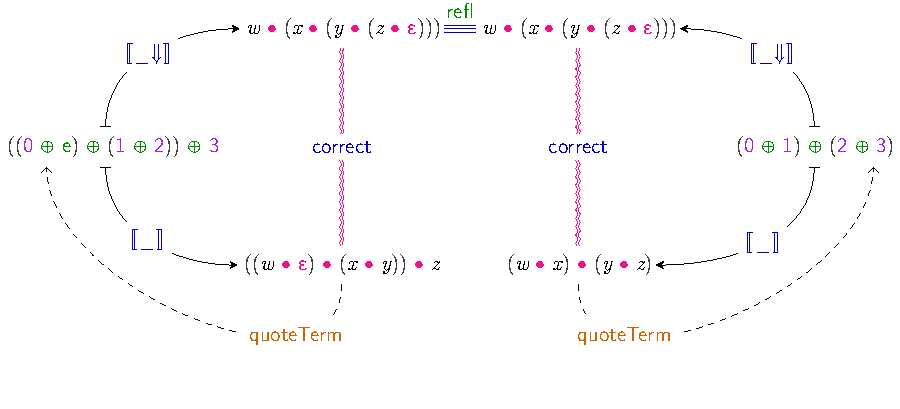
\includegraphics[draft=false]{graphics/reflexive-process}}
  \vspace*{-50pt}
  \caption{The Reflexive Proof Process}
  \label{proof-process}
\end{figure}
\begin{wrapfigure}{r}{0.6\textwidth}
  \vspace{-18pt}
  \ExecuteMetaData[ReflectionSection.tex]{expr-def}
  \caption{A Type for Ring Expressions}
  \label{expr}
\end{wrapfigure}

Before diving into to specifics, we'll first give a quick overview of how the
solver works, so it's clear how the bits of implementation described later in
the paper fit together.

The technique we use for automating equivalence proofs comes from
\cite{boutin_using_1997}: the general idea is that we prove two expressions
equivalent by proving that they're both equivalent to the same canonical form.
The diagram in Fig.~\ref{proof-process} demonstrates this for the identity from
Fig.~\ref{comparison}: on the bottom of the diagram you can see the left and
right hand side of the identity we want to prove, and on the top we can see
their normal forms. The actual proof the solver provides is represented by the
\(\AgdaField{≈}\) path.

To prove that each expression is equivalent to the canonical form we first
represent the expressions using the type in Fig.~\ref{expr}. This type
represents the Abstract Syntax Tree (AST) for expressions in the almost-ring
algebra: it has constructors corresponding to each ring operation (\(x + y = x
\; \AgdaInductiveConstructor{⊕} \; y\), \(x * y = x \;
\AgdaInductiveConstructor{⊗} \; y\)), and it can refer to variables via their de
Bruijn index (so \(x\) becomes \(\AgdaInductiveConstructor{I} \;
\AgdaNumber{0}\)).

There are two ways to evaluate the AST: the \(\AgdaFunction{⟦\_⟧}\) function
converts the AST to the expression we want to prove, whereas
\(\AgdaFunction{⟦\_⇓⟧}\) converts it to a the canonical form. The implementation
of the \(\AgdaFunction{⟦\_⇓⟧}\) function is described in
section~\ref{normalisation}.

Equivalence of the canonical forms is proven via \(\AgdaFunction{correct}\):
some of the details of this are explained in section~\ref{verif}.

Finally, instead of asking the user to construct the AST themselves, we use
reflection to automate it. This is described in the following section.
\section{The Interface} \label{interface}
\begin{figure}[b]
  \ExecuteMetaData[Introduction.tex]{old-solver}
  \caption{The Old Solver}
  \label{old-solver}
\end{figure}
\begin{wrapfigure}{r}{0.6\textwidth}
  \vspace{-18pt}
  \ExecuteMetaData[ReflectionSection.tex]{partial-auto}
  \caption{The \(\AgdaMacro{solveOver}\) Macro}
  \label{solveOver}
\end{wrapfigure}
We felt an easy-to-use interface was one of the most important components of the
library as a whole. Since we wanted to minimise the amount a user would have to
learn to use the solver, we kept the surface area of the library quite small:
aside from the almost-ring type, the rest of the interface consists of just two
macros (\(\AgdaMacro{solve}\) and \(\AgdaMacro{solveOver}\)). We tried to make
their usage as obvious as possible: just stick one of them (with the required
arguments) in the place you need a proof, and the solver will do the rest for
you.

\(\AgdaMacro{solve}\) is demonstrated in Fig.~\ref{the-solver}. It takes a
single argument: an implementation of the algebra. \(\AgdaMacro{solveOver}\) is
designed to be used in conjunction with manual proofs, so that a programmer can
automate a ``boring'' section of a larger more complex proof
(Fig.~\ref{solveOver}). As well as the algebra implementation, this macro takes
a list of free variables to use to compute the solution.

Because this interface is quite small, it's worth pointing out what's missing,
or rather, what we \emph{don't} require from the user:

\begin{itemize}
  \item We don't ask the user to construct the \(\AgdaDatatype{Expr}\) AST which
    represents their proof obligation. Compare this to Fig.~\ref{old-solver}: we
    had to write the type of the proof twice (once in the signature and again in
    the AST), and we had to learn the syntax for the solver's AST. 

    As well as being more verbose, this approach is less composable: every
    change to the proof type has to be accompanied by a corresponding change in
    the call to the solver. In contrast, the call to \(\AgdaMacro{solveOver}\)
    above effectively amounts to a demand for the compiler to ``figure it out!''
    Any change to the expressions on either side will result in an
    \emph{automatic} change to the proof constructed.
  \item We don't ask the user to write any kind of ``reflection logic'' for
    their type. In other words, we don't require a function which (for instance)
    recognises and parses the user's type in the reflected AST, or a function
    which does the opposite, converting a concrete value into the AST that (when
    unquoted) would produce an expression equivalent to the quoted value.

    This kind of logic is complex, and very difficult to get right. While some
    libraries can assist with the task \cite{hinze_engineering_2013,
      norell_agda-prelude_2018} it is still not fully automatic.

\end{itemize}
\subsection{Implementation} \label{reflection}
Agda has powerful metaprogramming facilities, which allow programs to manipulate
their own code. Here, we'll use reflection to implement the interface to our
solver.

Agda's reflection API is mostly encapsulated by the following three types:
\begin{description}
  \item[\(\AgdaDatatype{Term}\)] The representation of Agda's AST, retrievable
    via \(\AgdaKeyword{quoteTerm}\).
  \item[\(\AgdaDatatype{Name}\)] The representation of identifiers, retrievable
    via \(\AgdaKeyword{quote}\).
  \item[\(\AgdaDatatype{TC}\)] The type-checker monad, which includes scoping
    and environment information, can raise type errors, unify variables, or
    provide fresh names. Computations in the \(\AgdaDatatype{TC}\) monad can be
    run with \(\AgdaKeyword{unquote}\).
\end{description}

While \(\AgdaKeyword{quote}\), \(\AgdaKeyword{quoteTerm}\), and
\(\AgdaKeyword{unquote}\) provide all the functionality we need, they're
somewhat low-level and noisy (syntactically speaking). Agda also provides a
mechanism (which it calls macros) to package metaprogramming code so it looks
like a normal function call (as in \(\AgdaMacro{solve}\)).

Reflection is obviously a powerful tool, but it has a reputation for being
unsafe and error-prone. Agda's reflection system does not break type safety, but
we \emph{are} able to construct \(\AgdaDatatype{Term}\)s which are ill-typed,
which often result in confusing error-messages on the user's end. Unfortunately,
constructing ill-typed terms is quite easy to do: the \(\AgdaDatatype{Term}\)
type itself does not contain a whole lot of type information, and it's quite
fragile and sensitive to context. Variables, for instance, are referred to by
their de Bruijn indices, meaning that the same \(\AgdaDatatype{Term}\) can break
if it's simply moved under a lambda.

Building a robust interface using reflection required a great deal of care. To
demonstrate some of the techniques we used, we'll look at two functions from the
core of the interface. First, \(\AgdaFunction{toExpr}\):
\begin{center}
  \ExecuteMetaData[ReflectionSection.tex]{to-expr}
\end{center}
This function is called on the \(\AgdaDatatype{Term}\) representing one side of
the target equivalence. It converts it to the corresponding
\(\AgdaDatatype{Expr}\). In other words, it performs the following
transformation:
\[
  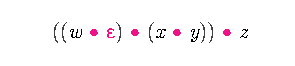
\includegraphics[trim={25 14 28 10}]{graphics/lhs-expr}
  \dashrightarrow
  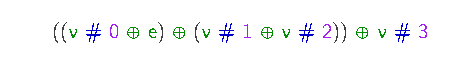
\includegraphics[trim={25 14 22 10}]{graphics/lhs-ast}
\]

When it encounters one of the ring operators, it calls the corresponding helper
function (\(\AgdaFunction{getBinOp}\), \(\AgdaFunction{getExp}\), or
\(\AgdaFunction{getUnOp}\)) which finds the important subterms from the
operator's argument list.

If it \emph{does not} manage to match an operator or a variable, it assumes that
what it has must be a constant, and wraps it up in the
\(\AgdaInductiveConstructor{K}\) constructor. This is the key trick which allows
us to avoid ever asking the user to quote their own type. While it may seem
unsafe at first glance, we actually found it to be more robust (for our use
case) than the alternative:
\begin{principle}[Don't reimplement the typechecker] While it may seem good and
  fastidious to rigorously check the structure and types of arguments given to a
  macro, we found better results by avoiding validity-checking in
  metaprogramming code. Instead, we preferred to proceed as if there were no
  errors (if possible), but arrange the output so that the user would still see
  a type error where the input was incorrect.

  Taking this case as an example, if the user indeed manages to supply something
  other than the correct type, Agda will catch the error, as an incorrect
  argument to \(\AgdaInductiveConstructor{K}\).

  If, on the other hand, we had asked the user to quote their own type, we
  would have trouble handling (for instance) closed applications of functions,
  references to names outside the lambda, etc. This approach, on the other hand,
  has no such difficulty.
\end{principle}

Next, we'll look at one of the helper functions: \(\AgdaFunction{getExp}\),
which deals with exponentiation.
\begin{center}
  \ExecuteMetaData[ReflectionSection.tex]{getExp}
\end{center}

It extracts the last two arguments to the exponentiation operator, and wraps
them up with the \(\AgdaInductiveConstructor{⊛}\). Before the two visible
arguments to the exponentiation operator, we first apply \(\AgdaNumber{3} \;
\AgdaFunction{⋯⟅∷⟆}\). This applies three hidden arguments as ``unknown'', i.e.
asks Agda to infer them. We could guess them ourselves: the first is the
universe level of the carrier type, the second is the carrier type, and the
third is the number of variables in the expression. We decided against it,
though, instead being intentionally unspecific:

\begin{principle}[Supply the minimal amount of information] There were several
  instances where, in constructing a term, we were tempted to supply explicitly
  some argument that Agda usually infers. Universe levels were a common example.
  We found this approach to be error-prone, however: as it turns out, the
  compiler is better a guessing implicits than we are. Instead, we preferred to
  \emph{leverage} the compiler, relying on inference over direct metaprogramming
  as much as possible.
\end{principle}

The final point to make is that the entire interface implementation is itself
quite small (fewer than 100 lines). This isn't because our code was terse:
rather, we intentionally minimised the amount of metaprogramming we did.

\begin{principle}[Keep Metaprogramming to the Edges] With great power comes poor
  error messages, fragility, and a loss of first-class status. Therefore, If
  something can be done without reflection, \emph{do it}, and use reflection as
  the glue to get from one standard representation to another.
\end{principle}
\subsection{Maintaining Invariants}
One obvious benefit of reflection is a terse interface. However, we feel that
another benefit---resilience to change---is just as important. This section
illustrates that resilience with an example.

Agda allows us to encode program correctness in types, so we can \emph{prove}
properties we would have otherwise only been able to test. Unfortunately, these
kinds of proofs tend to be very tightly coupled to the implementation of the
algorithms they verify. This can make iteration difficult, where small
optimisations or bug fixes can invalidate proofs for other invariants.

To demonstrate the problem, and how our solver can reduce some of the burden,
we'll look at size-indexed binary trees:
\begin{center}
  \ExecuteMetaData[Invariants.tex]{tree}
\end{center}

We've deliberately chosen an awkward type here: in contrast to the more common
size-indexed lists, the index (the size) does not match the shape of the data
structure. As a result, almost every function which manipulates the tree in some
way will have to come accompanied by a verbose, complex proof. Take this line,
for instance, which performs a left-rotation on the tree:
\begin{center}
  \ExecuteMetaData[Invariants.tex]{unproven}
\end{center}

A sensible invariant to encode here is that the function does not change the size
of the tree. Unfortunately, to \emph{prove} that invariant, we have to prove the
following:
\[1 + (1 + a + c) + b = 1 + a + (1 + b + c)\]

Though simple, this is precisely the kind of proof which requires many fussy
applications of the ring axioms. Here, our solver can help:
\begin{center}
  \ExecuteMetaData[Invariants.tex]{mistake}
\end{center}

While cutting down on the amount of code we need to write is always a good
thing, the real strength of this method is that it automatically infers the
input type. This makes it resilient to small changes in the code. So, when we
notice the bug in the code above (\(yl\) and \(yr\) are swapped in the
pattern-match), we can simply \emph{fix it}, without having to touch any of the
proof code.
\begin{center}
  \ExecuteMetaData[Invariants.tex]{correct}
\end{center}

If we hadn't used the solver, this fix would have necessitated a totally new
proof. By automating the proof, we allow the compiler to automatically check
what we \emph{mean} (``does the size of the tree stay the same?''), while we
worry about other details.
\section{Performance} \label{performance}
Our solver is significantly faster than the current solver: the following
sections will detail how we achieved that speedup. We will start by describing
the naive implementation; in section~\ref{sparse-opt} we demonstrate how we
added the optimisations from \cite{gregoire_proving_2005}; and in
section~\ref{syntactic-unif} we will describe the Agda-specific optimisations
which account for the bulk of our speedup. Finally, section~\ref{benchmarks}
contains some benchmarks against the current solver.
\subsection{Normalisation} \label{normalisation}
Most of code written for the solver is concerned with normalisation: the
\(\AgdaFunction{⟦\_⇓⟧}\) function in Fig.~\ref{proof-process}. This converts
from the expression AST (Fig.~\ref{expr}) to a canonical form.
\subsubsection{Horner Normal Form} \label{hnf}
The particular ``canonical form'' we'll start with is the same as in Agda's
current ring solver: Horner normal form. A polynomial (more specifically,
a monomial) in \(x\) is represented as a list of coefficients of increasing
powers of \(x\). As an example, the following polynomial:
\begin{align}
  3 + 2x^2 + 4x^5 + 2x^7 \label{example-poly}
\end{align}
Is represented by this list:
\begin{center}
  \ExecuteMetaData[HornerNormalForm.tex]{dense-example}
\end{center}
Operations on these polynomials are similar to operations in positional number
systems.
\begin{multicols}{2}
  \ExecuteMetaData[HornerNormalForm.tex]{impl}
\end{multicols}
So to get from \(\AgdaDatatype{Expr}\) to \(\AgdaDatatype{Poly}\) we map each
constructor to the relevant polynomial operation. Then, to get from
\(\AgdaDatatype{Poly}\) to an expression in the underlying ring, we use Horner's
rule: a classic example of the \(\AgdaFunction{foldr}\) function.
\begin{center}
  \ExecuteMetaData[HornerNormalForm.tex]{eval}
\end{center}
\subsubsection{Sparse Encodings} \label{sparse-opt}
Our first avenue for optimisation comes from \cite{gregoire_proving_2005}.
Notice that the encoding above is quite wasteful: it always stores an entry for
each coefficient, even if it's zero. In practice, we're likely to often find
long strings of zeroes (in expressions like \(x^{10}\)), meaning that our
representation will contain long ``gaps'' between the coefficients we're
actually interested in (non-zero ones).

To fix the problem we'll switch to a \emph{sparse} encoding, by storing a
``power index'' with every coefficient. This will represent the size of the gap
from the previous non-zero coefficient. Taking \ref{example-poly} again as an
example, we would now represent it as follows:
\begin{center}
  \ExecuteMetaData[HornerNormalForm.tex]{sparse-example}
\end{center}

Next, we turn our attention to the task of adding multiple variables. Luckily,
there's an easy way to do it: nesting. Multivariate polynomials will be
represented as ``polynomials of polynomials'', where each level of nesting
corresponds to one variable. It's perhaps more clearly expressible in types:
\begin{center}
  \ExecuteMetaData[HornerNormalForm.tex]{multi}
\end{center}
Inductively speaking, a ``polynomial'' in 0 variables is simply a constant,
whereas a polynomial in \(n\) variables is a list of coefficients, which are
themselves polynomials in \(n-1\) variables.

Before running off to use this representation, though, we should notice that we
have created another kind of ``gap'' which we should avoid with a sparse
encoding. For a polynomial with \(n\) variables, we will always have \(n\)
levels of nesting, even if the polynomial does not actually refer to all \(n\)
variables. In the extreme case, representing the constant \(6\) in a polynomial
of 3 variables looks like the following:
\begin{center}
  \ExecuteMetaData[HornerNormalForm.tex]{multi-nest}
\end{center}

The solution is another index: this time an ``injection'' index. This represents
``how many variables to skip over before you get to the interesting stuff''. In
contrast to the previous index, though, this one is type-relevant: we can't just
store a \(\Nat\) next to the nested polynomial to represent the gap. Because the
polynomial is indexed by the number of variables it contains, any encoding of
the gap will have provide the proper type information to respect that index.
\subsubsection{Hanging Indices}
The problem is a common one: we have a piece of code that works efficiently,
and we now want to make it ``more typed'', by adding more information to it,
\emph{without} changing the complexity class.

We found the following strategy to be useful: first, write the untyped version
of the code, forgetting about the desired invariants as much as possible. Then,
to add the extra type information, look for an inductive type which participates
in the algorithm, and see if you can ``hang'' some new type indices off of it.

In our case, the injection index (distance to the next ``interesting''
polynomial) was simply stored as an \(\Nat\), and the information we
needed was the number of variables in the inner polynomial, and the number of
variables in the outer. All of that is stored in the following proof of \(\le\):

\begin{center}
  \ExecuteMetaData[EfficiencyInIndexedTypes.tex]{leq-3}
\end{center}

A value of type \(n \; \AgdaDatatype{≤} \; m\) mimics the inductive structure of
the \(\Nat\) we were storing to represent the distance between \(n\)
and \(m\). We were able to take this analogy quite far: in a few functions, for
instance, we needed to compare these gaps. By mimicking the inductive structure
of \(\Nat\), we were able to directly translate \(\AgdaDatatype{Ordering}\) and
\(\AgdaFunction{compare}\) on \(\Nat\):

\begin{center}
  \ExecuteMetaData[EfficiencyInIndexedTypes.tex]{ord-type}
\end{center}

into equivalent functions on \(\le\):

\ExecuteMetaData[EfficiencyInIndexedTypes.tex]{leq-compare}
\subsection{Unification} \label{syntactic-unif}
After applying the previous optimisations, we might expect an immediate speedup
in the solver: unfortunately, this isn't the case. Without some careful
adjustments, the optimisations in the previous section can actually \emph{slow
  down} the solver. In this section, we'll try and explain the problem and how
we fixed it, and give general guidelines on how to write Agda code which
typechecks quickly.

Up until now, we have focused on the \emph{operations} performed on the
polynomial. Remember, though, the reflexive proof process has several steps:
only one of them containing the operations (\(\AgdaFunction{⟦\_⇓⟧}\) in
Fig.~\ref{proof-process}). Despite having the most complex implementation, this
isn't the most expensive step: surprisingly, the innocuous-looking
\(\AgdaInductiveConstructor{refl}\) takes the bulk of the time! Typechecking
this step involves unifying the two normalised expressions, a task which is
quite expensive, with counterintuitive performance characteristics.  

First, the good news. In the general case, unifying two expressions takes time
proportional to the size of those expressions, so our hard-won optimisations do
indeed help us.

Unfortunately, though, the ``general case'' isn't really that general: Agda's
unification algorithm has a very important shortcut which we \emph{must} make
use of if we want our code to typecheck quickly: \emph{syntactic equality}.

Before the full unification algorithm, Agda runs a quick check to see if the two
expressions it's testing for equality are \emph{syntactically} equal. This can
make a big difference in unification problems like the following:
\[ \AgdaFunction{sum} \; [ \AgdaNumber{1} .. \AgdaNumber{100} ] \stackrel{?}{=}
  \AgdaFunction{sum} \; [ \AgdaNumber{1} .. \AgdaNumber{100} ] \]

By noticing that these expressions are syntactically equal, we can avoid
actually computing the \(\AgdaFunction{sum}\) function. Taking advantage of that
shortcut is key to achieving decent performance. With that in mind, there are
two main strategies we'll use to encourage syntactic equality:
\subsubsection{Avoid Progress at all Costs}
First, we will consider something which may seem inconsequential: the order of
arguments to the evaluation functions.
\ExecuteMetaData[PerformanceOfTypeChecking.tex]{forwards-eval}
\ExecuteMetaData[PerformanceOfTypeChecking.tex]{backwards-eval}
\(\AgdaFunction{⟦\_⟧ₗ}\) is the definition we've been working with so far. Some
readers might find \(\AgdaFunction{⟦\_⟧ᵣ}\) more natural, however. The reason is
that it's more productive: in lazy languages, the usual convention is that
functions which take multiple arguments should scrutinise those arguments from
left to right. The \(\AgdaFunction{*}\) and \(\AgdaFunction{+}\) functions (on
\(\Nat\), at any rate) follow that convention, meaning that
\(\AgdaFunction{⟦\_⟧ᵣ}\) is able to make more progress without a concrete \(x\).
Taking the polynomial \(x^2 + 2\) as an example:
\begin{multicols}{2}
  \ExecuteMetaData[PerformanceOfTypeChecking.tex]{for-progress}
  \ExecuteMetaData[PerformanceOfTypeChecking.tex]{back-progress}
\end{multicols}
In \(\AgdaFunction{⟦\_⟧ₗ}\), we're blocked pretty much straight away, as \(x\)
is the first thing we try to scrutinise. In \(\AgdaFunction{⟦\_⟧ᵣ}\), since all
of the constants are kept to the left, they're scrutinised first, allowing us to
perform much more normalisation before being blocked.

This is exactly what you \emph{don't} want! Since both expressions
will be coming out of the same evaluation function, they should have the same
structure, meaning that we don't \emph{need} the reduction of outer terms that
\(\AgdaFunction{⟦\_⟧ᵣ}\) gives us. We only need to perform normalisation on the
coefficients: these are computed during the manipulations of the polynomial, and
so may contain unevaluated expressions. If we used \(\AgdaFunction{⟦\_⟧ᵣ}\) as
our definition, then the type checker will likely hit an inequality on the
\emph{first} term, and as a result we lose all opportunity for syntactic
equality. \(\AgdaFunction{⟦\_⟧ₗ}\), on the other hand, front-loads all of the
variables, maintaining syntactic equality for as long as possible.

As well as that, we don't have any control of the structure we get from the ring
operators. This means that any reduction, as well as being unnecessary, can
destroy the structural similarity between the two expressions, and as a result
their syntactic equality.

The (counterintuitive) lesson learned is as follows: to speed up unification,
keep things which are likely to be syntactically equal to the left, and
\emph{don't} structure your functions to encourage progress. Simply swapping the
arguments (as we do above) resulted in a performance improvement of several
orders of magnitude.
\subsubsection{Avoid Identities}

\begin{figure}[h]
  \centering
  \vspace{-50pt}
  \begin{subfigure}{0.4\textwidth}
    \centering
    \vspace{-10pt}
    \ExecuteMetaData[PerformanceOfTypeChecking.tex]{small-force}
    \caption{Sparse encoding, with identity-avoiding optimisation}
  \end{subfigure}
  \begin{subfigure}{0.4\textwidth}
    \centering
    \vspace{-10pt}
    \ExecuteMetaData[PerformanceOfTypeChecking.tex]{dense-term}
    \caption{Dense encoding, without identity-avoiding optimisation}
  \end{subfigure}
  \caption{Comparison of the normal forms of equation~\ref{example-poly}}
  \label{normal-forms}
\end{figure}

It's a good idea to avoid identities (expressions like \(0 + x\) or \(1 * x\))
in the normalised expression. This will reduce the size of your expression,
which is helpful in general, but more importantly it increases the likelihood of
finding syntactic equality in the argument to the identity (\(x\) in the
examples above). \pagebreak

Our sparse representation helps significantly in this case by entirely removing
\(\AgdaNumber{0}\) from the generated expression. Another place we can make
improvements is in the base cases for recursive functions. Take exponentiation,
for example:
\begin{center}
  \ExecuteMetaData[PerformanceOfTypeChecking.tex]{pow-bad}
\end{center}
We can avoid that \(\AgdaNumber{1}\) in the majority of cases by rewriting the
function to have an extra base case:
\begin{multicols}{2}
  \centering
  \ExecuteMetaData[PerformanceOfTypeChecking.tex]{pow-ident}
\end{multicols}
In the library, we employ this idea extensively, avoiding unnecessary identities
as much as we could. This has a significant effect on the size of the resulting
normal form, but also ensures that normalisation stops exactly where we want it
to, preserving the structure of the expressions as much as is possible. This
makes a significant difference to both size and syntactic
similarity as can be seen in Fig.~\ref{normal-forms}.
\subsection{Benchmarks} \label{benchmarks}
\begin{figure}[h]
  \newcounter{realxtickpos}
  \pgfplotsset{
      tick label style={font=\scriptsize},
      extra y tick style={yticklabel pos=right},
      title style={at={(-0.03,1.05)},anchor=west},
      xticklabel={%
        \ifnum \value{realxtickpos}=0%
          {$d = \pgfmathprintnumber{\tick}$}
        \else
          {$\pgfmathprintnumber{\tick}$}
        \fi
        \stepcounter{realxtickpos}
      },
      width=1.2\textwidth,
  }
  \setcounter{realxtickpos}{0}
  \begin{subfigure}[t]{0.3\textwidth}
    \begin{tikzpicture}
      \begin{axis}[
        % transpose legend,
        legend columns=1,
        legend entries={new, old},
        legend to name=benchplots,
        extra y ticks={15},
        title={(\subref{bench1}) $(x_1 + x_2 + \ldots + x_n)^d$},
        ]
        \addplot[color=blue, densely dashed] table {benchmark-data/sparse1.dat};
        \addplot[color=red] table {benchmark-data/dense1.dat};
      \end{axis}
    \end{tikzpicture}
    \phantomcaption \label{bench1}
  \end{subfigure}
  \setcounter{realxtickpos}{0}
  \begin{subfigure}[t]{0.3\textwidth}
    \begin{tikzpicture}
      \begin{axis}[
        extra y ticks={5},
        title={(\subref{bench2}) $x_1^d + x_2^d + \ldots + x_n^d$},
        ]
        \addplot[color=blue, densely dashed] table {benchmark-data/sparse2.dat};
        \addplot[color=red] table {benchmark-data/dense2.dat};
      \end{axis}
    \end{tikzpicture}
    \phantomcaption\label{bench2}
  \end{subfigure}
  \setcounter{realxtickpos}{0}
  \begin{subfigure}[t]{0.3\textwidth}
    \begin{tikzpicture}
      \begin{axis}[
        extra y ticks={40},
        title={(\subref{bench3}) $(x_1^n + x_2^{n-1} + \ldots + x_n^1 + 1)^d$},
        ]
        \addplot[color=blue, densely dashed] table {benchmark-data/sparse3.dat};
        \addplot[color=red] table {benchmark-data/dense3.dat};
      \end{axis}
    \end{tikzpicture}
    \phantomcaption\label{bench3}
  \end{subfigure}
  \begin{minipage}{0.13\textwidth}
    \vspace{-20pt}
    \ref{benchplots}
  \end{minipage}%
  \begin{minipage}{0.87\textwidth}
    \vspace{-20pt}
    \begin{flushleft}
      \caption{Time (in seconds) to prove each expression is equal to its expanded
        form ($n = 5$ for each).}
      \smallskip
      \footnotesize
      Benchmarks performed on Agda version 2.6-0fa9b13, with the Agda standard
      library at commit-3bd3334a9552490e396f73f96812105a27e5917b, on a 2016
      MacBook Pro, with a 2.9 GHz Intel Core i7 and 16 GB of RAM.
    \end{flushleft}
  \end{minipage} 
\end{figure}

As expected, the new implementation exhibits a significant speedup in
type-checking over the old implementation, even with the added overhead of the
reflection-based interface. Fig.~\ref{bench1} shows time taken to type check a
proof that \((x_1 + x_2 + x_3 + x_4 + x_5)^d\) is equal to its expanded form.
The new representation is clearly faster overall, with a factor of 7.5
speedup for \(d = 8\).

Fig.~\ref{bench3} demonstrates perhaps a more common use-case, with a mix of
high and low powers and some constants. The new representation's advantage is
even more apparent here, with an \(30\)-factor speedup at \(d = 8\).

The old solver does exhibit a small lead (roughly 2-3 seconds, which narrows
to about 1 second without reflection) on very simple expressions, possibly
caused by the overhead of the new solver's more complex implementation. 3
seconds is quite small in the context of Agda type checking (the standard
library, for instance, takes several minutes to type check), so we feel this
slight loss is more than made up for by the gains. Furthermore,
we have not been able to find a case where the old solver is significantly
faster than the new. Nonetheless, if a user really wants to use the old
solver, the other components described here are entirely modular, and can work
with any underlying solver which uses the reflexive technique.

\section{Verification} \label{verif}
The output of the solver is a constructive proof of equivalence: this is
\emph{derived} from a generic proof that the operations on the solver are a ring
homomorphism from the carrier type. Put another way, for the solver to work
properly, we would need to prove that addition (and multiplication, and
negation, etc.) on Horner normal forms corresponds with addition on the carrier
type.

These proofs are long (about 1000 lines) and complex. Without careful
structuring of the proofs, every new optimisation would require a whole new
round of proof code, with very little reuse.

To avoid this problem, we took inspiration from \cite{mu_algebra_2009}, and
relied heavily on abstraction and folds to improve the reuse in proof code. In
particular, we defined many operations as \emph{metamorphisms}
\cite{gibbons_metamorphisms_2007}. So, instead of defining (say) negation over
the polynomial type itself, we will define a metamorphism to express negation,
and then call some higher-order function to run that metamorphism over a
polynomial.
\begin{center}
  \ExecuteMetaData[AbstractionAndFolds.tex]{fold-def}
\end{center}

\begin{wrapfigure}{r}{0.4\textwidth}
  \vspace{-18pt}
  \ExecuteMetaData[AbstractionAndFolds.tex]{poly-mapR}
  \caption{The Semantics of \(\AgdaFunction{poly-map}\)}
  \label{poly-map}
  \vspace{-15pt}
\end{wrapfigure}

From here, we can define the \emph{semantics} of a metamorphism. As an example,
Fig.~\ref{poly-map} shows the semantics of \(\AgdaFunction{poly-map}\), a simple
morphism which behaves something like \(\AgdaFunction{map}\) on lists.

Now, each operation only has to be proven up to the semantics defined above.
Crucially, optimisations like the sparse encoding \emph{respect} these
semantics, so we only have to change our proof in one place: the definition of
\(\AgdaFunction{poly-mapR}\).
\section{Pedagogical Solutions} \label{pedagogical}
One of the core aims of this work is to take a step towards making Agda a useful
tool for doing mathematics. The rest of this paper has described our efforts to
compensate for Agda's disadvantage in this area: namely, a pedantic typechecker.
This section will attempt to show the other side of the coin, and demonstrate
some of the unique benefits that come from using a programming language to do
your proofs.

Outside of computer scientists and mathematicians, most people's experience of
computer algebra probably amounts to the step-by-step solutions from
Wolfram|Alpha \cite{the_development_team_step-by-step_2009} or some similar
system. 

Something so high-level and user-facing hardly seems like it's in a
dependently-typed language's wheelhouse; on the other hand, the very nature of a
proof in Agda is that it has computational content: why not make some of that
content an explanation for the equality?

Prior work in this area includes \cite{lioubartsev_constructing_2016}: there,
the problem is reformulated  reformulates the problem as one of
\emph{path-finding}. The left-hand-side and right-hand-side of the equation are
vertices in a graph, where the edges are single steps to rewrite an expression
to an equivalent form. A* is used to search.

Unfortunately, this approach has to deal with a huge search space: every vertex
will have an edge for almost every one of the ring axioms, and as such a good
heuristic is essential. Furthermore, what this should be is not clear:
\cite{lioubartsev_constructing_2016} uses a measure of the ``simplicity'' of an
expression.

\begin{wrapfigure}{r}{0.35\textwidth}
  \vspace{-10pt}
  \resizebox{0.35\textwidth}{!}{
    \begin{tikzpicture}
      \node (n0) at (2,9) {$1 + 2 + y + x$};
      \node (n1) at (-2,6) {$x + y * 1 + 3$};
      \node (n2) at (2,7.5) {$3 + y + x$};
      \node (n3) at (2,6) {$y + 3 + x$};
      \node (n4) at (0,4.5) {$x + y + 3$};
      \node (n5) at (-1,3) {$3 + x + y$};
      \node (n6) at (1,3) {$x + 3 + y$};
      \draw[-stealth] (n1) to (n4);
      \draw[-stealth] (n3) to (n2);
      \draw[-stealth] (n2) to (n0);
      \draw[-stealth] (n4) to (n3);
      \draw[-stealth] (n4) to (n5);
      \draw[-stealth] (n5) to (n6);
      \draw[-stealth] (n6) to (n4);
    \end{tikzpicture}
  }
  \vspace{-15pt}
  \caption{Graph Containing Loops}
  \label{h-graph}
  \vspace{-20pt}
\end{wrapfigure}


Notice, however, that paths in undirected graphs form a perfectly reasonable
equivalence relation: transitivity is the concatenation of paths, reflexivity is
the empty path, and symmetry is \emph{reversing} a path. Equivalence classes, in
this analogy, are connected components of the graph.

More practically speaking, we implement these ``paths'' as lists, where the
elements of the list are elementary ring axioms. When we want to display a
step-by-step solution, we simply print out each element of the list in turn,
interspersed with the states of the expression (the vertices in the graph).

If we stopped there, however, the solver would output incredibly verbose
``solutions'': far too verbose to be human-readable. Instead, we must apply a
number of path-compression heuristics to cut down on the solution length:

\begin{enumerate}
  \item First, we remove loops from the graph. Fig~\ref{h-graph} shows an
    example solution without this heuristic applied: it crosses the same point
    multiple times, creating useless steps in the output. In contrast to
    using just A* on its own, the search space is minimal (with only one outward
    edge for each vertex).
  \item Then, we filter out ``uninteresting'' steps. These are steps which are
    obvious to a human, like associativity, or evaluation of closed terms. When
    a step is divided over two sides of an operator, it is deemed
    ``interesting'' if either side is interesting.
\end{enumerate}
After applying those heuristics, our solver outputs the explanation in
Fig.~\ref{step-output} for the lemma in Fig.~\ref{comparison}
\begin{figure}[h!]
  \centering
  \vspace{-10pt}
\begin{BVerbatim}
x + y + 3
    ={ +-comm(x, y + 3) }
y + 3 + x
    ={ +-comm(y, 3) }
3 + y + x
\end{BVerbatim}
  \caption{Step-by-Step Output From Our Solver}
  \label{step-output}
\end{figure}
\section{Related Work}
In dependently-typed programming languages, the state-of-the-art solver for
polynomial equalities (over commutative rings) was originally presented
in \cite{gregoire_proving_2005}, and is used in Coq's \verb+ring+ solver. This
work improved on the already existing solver \cite{Coq:manual} in both efficiency
and flexibility. In both the old and improved solvers, a reflexive technique is
used to automate the construction of the proof obligation (as described in
\cite{boutin_using_1997}).

Agda \cite{norell_dependently_2008} is a dependently-typed programming language
based on Martin-Löf's Intuitionistic Type
Theory \cite{martin-lof_intuitionistic_1980}. Its standard
library \cite{danielsson_agda_2018} currently contains a ring solver which is
similar in flexibility to Coq's \verb+ring+, but does not support the
reflection-based interface, and is less efficient to the one presented here. 

In \cite{geuvers_automatically_2017}, an implementation of an automated solver
for the dependently-typed language Idris \cite{brady_idris_2013} is described.
The solver is implemented with a ``correct-by-construction'' approach, in
contrast to \cite{gregoire_proving_2005}. The solver is defined over
\emph{non}commutative rings, meaning that it is more general (can work with more
types) but less powerful (meaning it can prove fewer identities). It provides a
reflection-based interface, but internally uses a dense representation.

Reflection and metaprogramming are relatively recent additions to Agda, but form
an important part of the interfaces to automated proof procedures. Reflection in
dependent types in general is explored in \cite{christiansen_practical_2015},
and specific to Agda in \cite{van_der_walt_reflection_2012}.

Formalisation of mathematics in general is an ongoing project.
\cite{wiedijk_formalizing_2018} tracks how much of ``The 100 Greatest Theorems''
\cite{kahl_hundred_2004} have so far been formalised (at time of writing, the
number stands at 93). DoCon \cite{meshveliani_docon-provable_2018} is a notable
Agda library in this regard: it contains many tools for basic maths, and
implementations of several CAS algorithms. Its implementation is described
in \cite{meshveliani_dependent_2013}. \cite{cheng_functional_2018} describes the
manipulation of polynomials in both Haskell and Agda.

Finally, the study of \emph{pedagogical} CASs which provide step-by-step
solutions is explored in \cite{lioubartsev_constructing_2016}. One of the most
well-known such system is Wolfram Alpha
\cite{wolfram_research_inc._wolframalpha_2019}, which has step-by-step solutions
\cite{the_development_team_step-by-step_2009}.

\section{Conclusion}
We have presented an efficient, flexible, and easy-to-use ring solver in the
programming language Agda. In doing so, we hope we have removed one of the small
but significant pain points of doing maths in Agda.

\bibliographystyle{plain}
\bibliography{bibliography.bib}

\end{document}
